
\begin{figure}
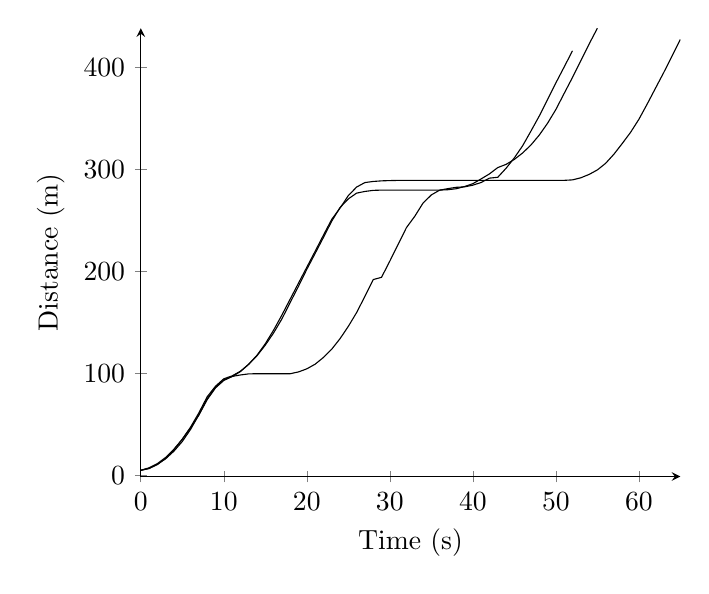
\begin{tikzpicture}
\begin{axis}[
legend style={anchor=west},
axis x line=bottom,
axis y line=left,
ymin=-1,
xlabel=Time (s),
ylabel=Distance (m),
]
\addplot[] coordinates {
(0, 5.1)
(1, 6.88912325064)
(2, 11.0339682318)
(3, 16.4502795601)
(4, 23.8890709832)
(5, 33.2917112911)
(6, 45.1805845519)
(7, 59.5439965158)
(8, 75.2672176143)
(9, 86.3478202624)
(10, 93.6963764927)
(11, 96.8745825244)
(12, 101.783358839)
(13, 108.964732427)
(14, 117.78057445)
(15, 129.077662661)
(16, 142.406545871)
(17, 157.191405476)
(18, 172.840121363)
(19, 188.464840843)
(20, 204.013790989)
(21, 219.560635088)
(22, 235.366790161)
(23, 250.884985002)
(24, 261.918404323)
(25, 274.148398304)
(26, 282.561651889)
(27, 286.956739058)
(28, 288.034141461)
(29, 288.632025391)
(30, 288.896377131)
(31, 289.076583874)
(32, 289.106258197)
(33, 289.128179356)
(34, 289.128179356)
(35, 289.128179356)
(36, 289.128179356)
(37, 289.128179356)
(38, 289.128179356)
(39, 289.128179356)
(40, 289.128179356)
(41, 289.128179356)
(42, 289.128179356)
(43, 289.128179356)
(44, 289.128179356)
(45, 289.128179356)
(46, 289.128179356)
(47, 289.128179356)
(48, 289.128179356)
(49, 289.128179356)
(50, 289.128179356)
(51, 289.128179356)
(52, 289.578124295)
(53, 291.619020144)
(54, 294.899890859)
(55, 299.347065372)
(56, 305.847761398)
(57, 314.811541234)
(58, 325.251023448)
(59, 336.165519727)
(60, 348.903474606)
(61, 363.854180986)
(62, 379.372463262)
(63, 394.846770967)
(64, 410.959448629)
(65, 427.149180057)
};
\addplot[] coordinates {
(0, 5.1)
(1, 6.88691925277)
(2, 10.7021701064)
(3, 16.764035256)
(4, 25.1937546883)
(5, 35.6355185652)
(6, 47.4099110095)
(7, 61.3943556375)
(8, 77.1258127628)
(9, 87.455858952)
(10, 94.7345185089)
(11, 97.5910355588)
(12, 102.137343983)
(13, 108.927384117)
(14, 117.329920224)
(15, 127.705782504)
(16, 139.676856159)
(17, 153.3890492)
(18, 169.511707464)
(19, 185.370974888)
(20, 201.939915056)
(21, 217.498132833)
(22, 233.169315728)
(23, 249.102449855)
(24, 262.483197022)
(25, 270.958505642)
(26, 276.61941801)
(27, 278.25472672)
(28, 279.314232499)
(29, 279.561609203)
(30, 279.586419287)
(31, 279.586419287)
(32, 279.586419287)
(33, 279.586419287)
(34, 279.586419287)
(35, 279.586419287)
(36, 279.586419287)
(37, 279.964395461)
(38, 280.913667706)
(39, 283.062304226)
(40, 285.843293681)
(41, 290.542254367)
(42, 295.456883845)
(43, 301.62866097)
(44, 304.76980037)
(45, 309.646079438)
(46, 315.957332525)
(47, 323.775252904)
(48, 333.465810984)
(49, 345.044651038)
(50, 358.511785019)
(51, 374.280531677)
(52, 389.860656971)
(53, 406.246310881)
(54, 422.554921208)
(55, 438.137115771)
};
\addplot[] coordinates {
(0, 5.1)
(1, 7.56303877706)
(2, 11.6166758586)
(3, 17.7688114941)
(4, 25.8696739369)
(5, 35.444041716)
(6, 46.5722712385)
(7, 59.2168207393)
(8, 74.2897793559)
(9, 85.8263375934)
(10, 93.0977708892)
(11, 97.0403642751)
(12, 98.4809926122)
(13, 99.568375934)
(14, 99.6981860806)
(15, 99.7155222697)
(16, 99.7155222697)
(17, 99.7155222697)
(18, 99.7155222697)
(19, 101.468554806)
(20, 104.486239858)
(21, 109.034393829)
(22, 115.632152122)
(23, 123.739220508)
(24, 134.014882108)
(25, 146.065188007)
(26, 159.632971089)
(27, 175.491280051)
(28, 191.935490857)
(29, 194.135046982)
(30, 210.031165371)
(31, 226.392633049)
(32, 242.80841335)
(33, 253.860650933)
(34, 266.848597955)
(35, 274.849700467)
(36, 279.513410653)
(37, 281.020146747)
(38, 282.306687978)
(39, 282.750842371)
(40, 284.385068486)
(41, 287.038817494)
(42, 291.300180755)
(43, 292.102844024)
(44, 300.951358088)
(45, 311.16316276)
(46, 323.046210844)
(47, 337.39791088)
(48, 352.141424157)
(49, 368.296750605)
(50, 384.571840179)
(51, 400.157279619)
(52, 416.00179607)
};

\end{axis}
\end{tikzpicture}
\label{tik:distance:0:31}
\caption{0 percent diving with GSC on route $31$}
\end{figure}
